%!TEX program = xelatex
\documentclass[11pt]{beamer}

\usepackage{amsfonts}
\usepackage{amsmath}
\usepackage{blindtext}
\usepackage{enumitem}
\usepackage{fancyvrb}
\usepackage{tikz}

\usetheme{SaoPaulo}  % can use SaoPaulo as well

\title{MATLAB}
\subtitle{Applications:  Statistics}
\author{CS101 Lecture \#25}
\date{2016-12-05}

\setcounter{showSlideNumbers}{1}

\newcommand{\correctstar}{{\Large\textcolor{red}{$\star$}}}

\begin{document}
  \setcounter{showProgressBar}{0}
  \setcounter{showSlideNumbers}{0}

%%%%%%%%%%%%%%%%%%%%%%%%%%%%%%%%%%%%%%%%%%%%%%%%%%%%%%%%%%%%%%%%%%%%%%%%%%%%%%%%
\frame{\titlepage}

%%%%%%%%%%%%%%%%%%%%%%%%%%%%%%%%%%%%%%%%%%%%%%%%%%%%%%%%%%%%%%%%%%%%%%%%%%%%%%%%
\setcounter{framenumber}{0}
\setcounter{showProgressBar}{1}
\setcounter{showSlideNumbers}{1}

%%%%%%%%%%%%%%%%%%%%%%%%%%%%%%%%%%%%%%%%%%%%%%%%%%%%%%%%%%%%%%%%%%%%%%%%%%%%%%%%
\section{Administrivia}

%%%%%%%%%%%%%%%%%%%%%%%%%%%%%%%%%%%%%%%%%%%%%%%%%%%%%%%%%%%%%%%%%%%%%%%%%%%%%%%%
\begin{frame}
  \frametitle{Administrivia}
  \Enlarge

   \begin{itemize}
   	\myitem  Homework \#12 is due Friday, Jan.\ 13.  %\pause
   %	\myitem  No lab \emph{t} week.  %\pause
   	\myitem  Final examination will be held Jan.\ 20, Friday 8am-11am in A-0414.  %\pause
   	% \myitem  Grade check period coming up:  Dec.\ 9--14.  \textcolor{CS101Base}{All Compass grades will be considered final after this.}
   \end{itemize}
\end{frame}

%%%%%%%%%%%%%%%%%%%%%%%%%%%%%%%%%%%%%%%%%%%%%%%%%%%%%%%%%%%%%%%%%%%%%%%%%%%%%%%
\begin{frame}[fragile]
	\frametitle{Recall: Matrix Indexing and Plot}
	%\Enlarge
	
	\begin{enumerate}
		\myitem  To refer to multiple elements of an array, use the colon operator to specify a range of the form start:end. 
		\begin{enumerate}
			\mysubitem  A(1:3,2) first 3 rows, 2nd column
			\mysubitem  A(3,:)  all columns in 3rd row
		\end{enumerate}
		\myitem plot https://www.mathworks.com/help/matlab/ref/plot.html
		\myitem plot(Y) creates a 2-D line plot of the data in Y versus the index of each value. If Y is a matrix, then the plot function plots the columns of Y versus their row number. The x-axis scale ranges from 1 to the number of rows in Y.
		\myitem plot(X,Y) creates a 2-D line plot of the data in Y versus the corresponding values in X.
	\end{enumerate}
\end{frame}

%%%%%%%%%%%%%%%%%%%%%%%%%%%%%%%%%%%%%%%%%%%%%%%%%%%%%%%%%%%%%%%%%%%%%%%%%%%%%%%%
\section{Warmup Questions}

%%%%%%%%%%%%%%%%%%%%%%%%%%%%%%%%%%%%%%%%%%%%%%%%%%%%%%%%%%%%%%%%%%%%%%%%%%%%%%%%
\begin{frame}[fragile]
  \frametitle{Question \#1}
  \Enlarge

  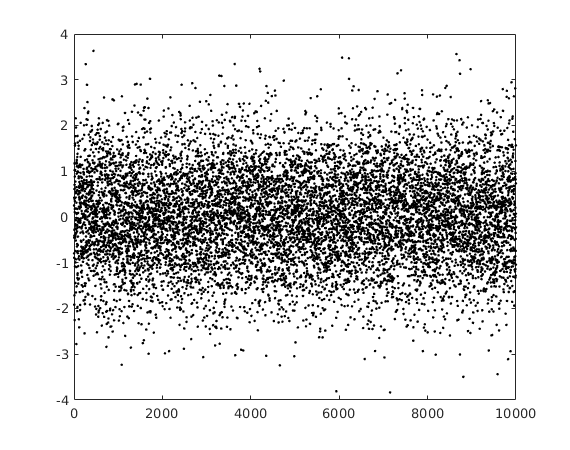
\includegraphics[width=0.33\textwidth]{./img/plot-normal.png}

Which of the following could produce this plot?

  \begin{enumerate}[label=\Alph*]
    \item
      \begin{Verbatim}
x = rand( 10000,1 );
      \end{Verbatim}
    \item
      \begin{Verbatim}
x = randi( 10000,1 );
      \end{Verbatim}
    \item
    \begin{Verbatim}
x = randn( 10000,1 );
    \end{Verbatim}
  \end{enumerate}
  ~
  \begin{Verbatim}
plot( x,'.' );
  \end{Verbatim}
\end{frame}

%%%%%%%%%%%%%%%%%%%%%%%%%%%%%%%%%%%%%%%%%%%%%%%%%%%%%%%%%%%%%%%%%%%%%%%%%%%%%%%%
\begin{frame}[fragile]
  \frametitle{Question \#1}
  \Enlarge

  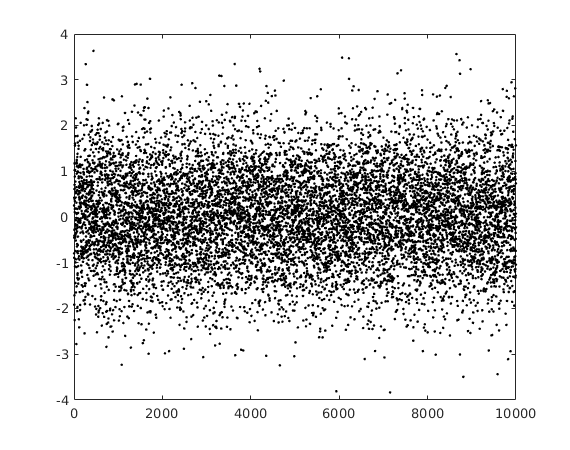
\includegraphics[width=0.33\textwidth]{./img/plot-normal.png}

Which of the following could produce this plot?

  \begin{enumerate}[label=\Alph*]
    \item
      \begin{Verbatim}
x = rand( 10000,1 );
      \end{Verbatim}
    \item
      \begin{Verbatim}
x = randi( 10000,1 );
      \end{Verbatim}
    \item
    \begin{Verbatim}
x = randn( 10000,1 );
    \end{Verbatim}
    \correctstar
  \end{enumerate}
  \begin{Verbatim}
plot( x,'.' );
  \end{Verbatim}
\end{frame}

%%%%%%%%%%%%%%%%%%%%%%%%%%%%%%%%%%%%%%%%%%%%%%%%%%%%%%%%%%%%%%%%%%%%%%%%%%%%%%%%
\begin{frame}[fragile]
  \frametitle{Question \#2}
  \Enlarge

  $$
\underline{\underline{A}} \underline{x} = \underline{b}
  $$

Which is the preferred way to solve this matrix--vector equation?

  \begin{enumerate}[label=\Alph*]
    \item  \texttt{x = inv( A ) * b;}
    \item  \texttt{x = A \textbackslash ~b;}
    \item  \texttt{x = inv( A ) .* b;}
    \item  \texttt{x = A / b;}
  \end{enumerate}
\end{frame}

%%%%%%%%%%%%%%%%%%%%%%%%%%%%%%%%%%%%%%%%%%%%%%%%%%%%%%%%%%%%%%%%%%%%%%%%%%%%%%%%
\begin{frame}[fragile]
  \frametitle{Question \#2}
  %\Enlarge

  $$
\underline{\underline{A}} \underline{x} = \underline{b}
  $$

Which is the preferred way to solve this matrix--vector equation?

  \begin{enumerate}[label=\Alph*]
    \item  \texttt{x = inv( A ) * b;}  Why not this one?
    If A is a square matrix, A \textbackslash ~b is roughly equal to inv(A) * b, but MATLAB processes  A \textbackslash ~b differently and more robustly. https://www.mathworks.com/help/matlab/ref/mldivide.html
    https://www.mathworks.com/help/matlab/ref/inv.html
    \item  \texttt{x = A \textbackslash ~b;}  \correctstar
    \item  \texttt{x = inv( A ) .* b;}
    \item  \texttt{x = A / b;}
  \end{enumerate}
\end{frame}

%%%%%%%%%%%%%%%%%%%%%%%%%%%%%%%%%%%%%%%%%%%%%%%%%%%%%%%%%%%%%%%%%%%%%%%%%%%%%%%%
\begin{frame}[fragile]
  \frametitle{Question \#3}
  \Enlarge

  \begin{Verbatim}
A = [ 5 4 1- 2 2 ];
B = [ 5 4 1 -2 2 ];
  \end{Verbatim}

Are \texttt{A} and \texttt{B} equal in value?

  \begin{enumerate}[label=\Alph*]
    \item  Yes
    \item  No
  \end{enumerate}
\end{frame}

%%%%%%%%%%%%%%%%%%%%%%%%%%%%%%%%%%%%%%%%%%%%%%%%%%%%%%%%%%%%%%%%%%%%%%%%%%%%%%%%
\begin{frame}[fragile]
  \frametitle{Question \#3}
  \Enlarge

  \begin{Verbatim}
A = [ 5 4 1- 2 2 ];
B = [ 5 4 1 -2 2 ];
  \end{Verbatim}

Are \texttt{A} and \texttt{B} equal in value?

  \begin{enumerate}[label=\Alph*]
    \item  Yes
    \item  No  \correctstar
  \end{enumerate}
\end{frame}



%%%%%%%%%%%%%%%%%%%%%%%%%%%%%%%%%%%%%%%%%%%%%%%%%%%%%%%%%%%%%%%%%%%%%%%%%%%%%%%
\begin{frame}[fragile]
	\frametitle{Example:  Brexit polling}
	
	\begin{Verbatim}
    poll = csvread('brexit.csv');
    % poll is a matrix. 
    % In matlab, you can use 
    % poll = importdata(’brexit.csv’);
    % Then change below poll to be poll.data
    
    plot( poll(:,2) );
    plot( poll(:,3) );
    % oh no! our plotted data disappeared!
	\end{Verbatim}
\end{frame}

%%%%%%%%%%%%%%%%%%%%%%%%%%%%%%%%%%%%%%%%%%%%%%%%%%%%%%%%%%%%%%%%%%%%%%%%%%%%%%%
\begin{frame}[fragile]
	\frametitle{Example:  Brexit polling}
	
	\begin{Verbatim}
    poll = csvread('brexit.csv');
    hold on;  % make plots persistent until closed
    plot( poll(:,2) );
    plot( poll(:,3) );
    plot( poll(:,4) );
	\end{Verbatim}
\end{frame}

%%%%%%%%%%%%%%%%%%%%%%%%%%%%%%%%%%%%%%%%%%%%%%%%%%%%%%%%%%%%%%%%%%%%%%%%%%%%%%%
\begin{frame}[fragile]
	\frametitle{Example:  Brexit polling}
	
	\begin{Verbatim}
    n = numel(poll(:,2));
    
    mean_r = mean( poll(:,2) ) * ones( n+1,1 );
    stdev_r = std( poll(:,2) );
    std_rp = mean_r+stdev_r;
    std_rm = mean_r-stdev_r;
    hold on
    plot( poll(:,2), 'ro' );
    plot( 0:n,mean_r, 'r-' );
    plot( 0:n,std_rp, 'r--' );
    plot( 0:n,std_rm, 'r--' );
	\end{Verbatim}
\end{frame}

%%%%%%%%%%%%%%%%%%%%%%%%%%%%%%%%%%%%%%%%%%%%%%%%%%%%%%%%%%%%%%%%%%%%%%%%%%%%%%%
\begin{frame}[fragile]
	\frametitle{Example:  Brexit polling}
	
	\begin{Verbatim}
    n = numel(poll(:,2));
    mean_r = rolling_mean( poll(:,2)', 25 );
    stdev_r = rolling_std( poll(:,2)', 25 );
    std_rp = mean_r+stdev_r;
    std_rm = mean_r-stdev_r;
    hold on
    plot( poll(:,2), 'ro' );
    plot( 0:n-1,mean_r, 'r-' );
    plot( 0:n-1,std_rp, 'r--' );
    plot( 0:n-1,std_rm, 'r--' );
	\end{Verbatim}
\end{frame}

%%%%%%%%%%%%%%%%%%%%%%%%%%%%%%%%%%%%%%%%%%%%%%%%%%%%%%%%%%%%%%%%%%%%%%%%%%%%%%%%

%%%%%%%%%%%%%%%%%%%%%%%%%%%%%%%%%%%%%%%%%%%%%%%%%%%%%%%%%%%%%%%%%%%%%%%%%%%%%%%%
\section{Statistics}

%%%%%%%%%%%%%%%%%%%%%%%%%%%%%%%%%%%%%%%%%%%%%%%%%%%%%%%%%%%%%%%%%%%%%%%%%%%%%%%
\begin{frame}[fragile]
	\frametitle{Statistical quantities}
	%\Enlarge
	
	\begin{enumerate}
		\myitem  Many operations are available:
		\begin{enumerate}
			\mysubitem  \texttt{mean} (average), \texttt{median}, \texttt{std}
			\mysubitem  \texttt{max}, \texttt{min}, \texttt{range}
			\mysubitem  \texttt{iqr} (interquartile range), \texttt{corrcoef} (the correlation coefficient of two random variables is a measure of their linear dependence) (not yet supported in Octave but supported by https://octave.sourceforge.io/nan/function/corrcoef.html)
			\mysubitem  \texttt{sort}
			\mysubitem  \texttt{boxplot}, \texttt{hist}
		\end{enumerate}
	\end{enumerate}
\end{frame}

%%%%%%%%%%%%%%%%%%%%%%%%%%%%%%%%%%%%%%%%%%%%%%%%%%%%%%%%%%%%%%%%%%%%%%%%%%%%%%%
\begin{frame}[fragile]
  \frametitle{Statistical quantities}
  %\Enlarge

  \begin{enumerate}
  \myitem  Often we would like to \emph{fit} a set of data to an equation.  %\pause
  \myitem  We can then \emph{interpolate} or \emph{extrapolate}. 
  	\begin{enumerate}
     	\mysubitem  interpolate: to estimate a value within two known values in a sequence of values.
  		\mysubitem extrapolate: to infer something that is not explicitly stated from existing information. 	
    \end{enumerate}
   %\pause
  \myitem  This is called \emph{curve fitting} or \emph{regression}.
  \end{enumerate}

  \begin{columns}
    \begin{column}{0.33\textwidth}
    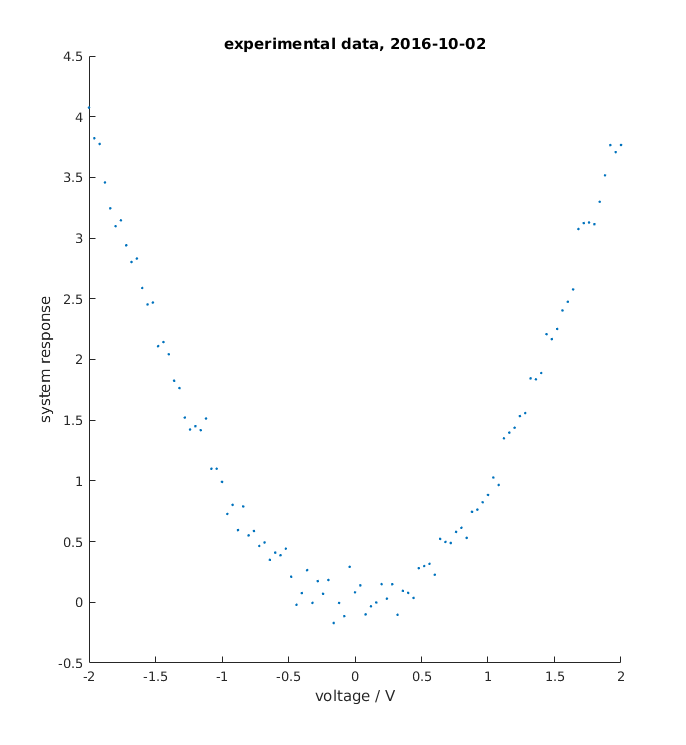
\includegraphics[width=\textwidth]{./img/expt1.png}
    \end{column}
    \begin{column}{0.33\textwidth}
    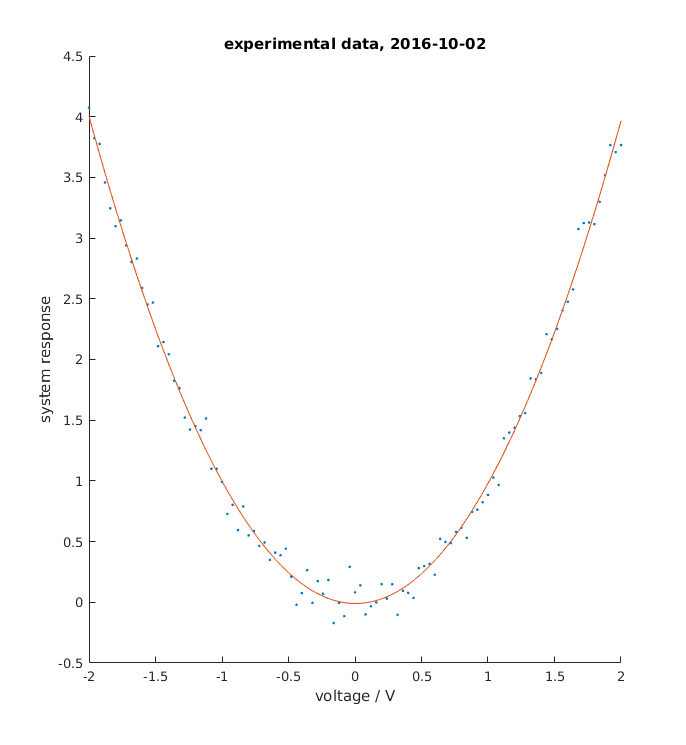
\includegraphics[width=\textwidth]{./img/expt2.png}
    \end{column}
  \end{columns}
\end{frame}

%%%%%%%%%%%%%%%%%%%%%%%%%%%%%%%%%%%%%%%%%%%%%%%%%%%%%%%%%%%%%%%%%%%%%%%%%%%%%%%
\begin{frame}[fragile]
  \frametitle{Statistical quantities}
  \Enlarge

  \begin{enumerate}
  \myitem  The simplest form of fitting is to a polynomial:
  \end{enumerate}
  $$
f(x) = a_{1} x^{3} + a_{2} x^{2} + a_{3} x + a_{4}
  $$
  %\pause
  \begin{enumerate}
  \myitem  (Note that the numbering is a bit odd!) %\pause
  \myitem  But first, we need to see how MATLAB represents polynomials.
  \end{enumerate}
\end{frame}

%%%%%%%%%%%%%%%%%%%%%%%%%%%%%%%%%%%%%%%%%%%%%%%%%%%%%%%%%%%%%%%%%%%%%%%%%%%%%%%
\begin{frame}[fragile]
  \frametitle{Polynomials}
  \Enlarge

  $$
a_{1} x^{3} + a_{2} x^{2} + a_{3} x + a_{4}
  $$
  \begin{Verbatim}
[ a1 a2 a3 a4 ]
  \end{Verbatim}
  %\pause
  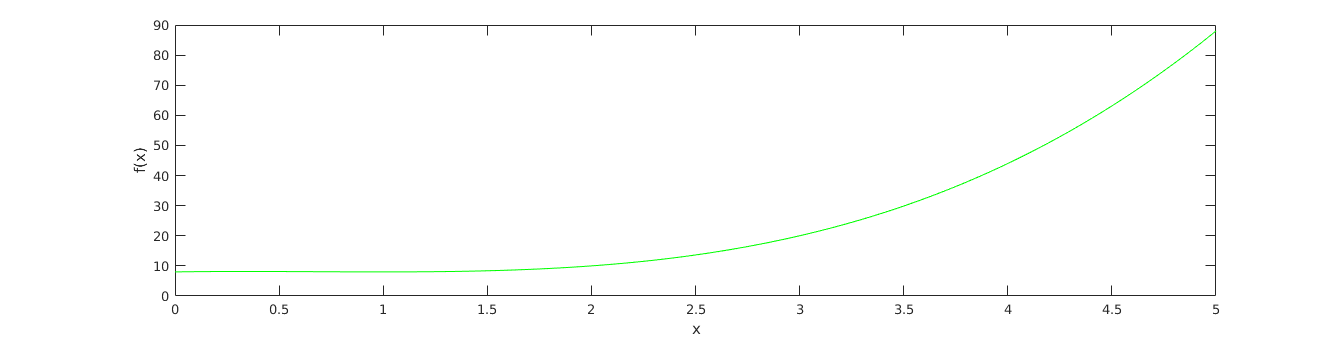
\includegraphics[width=0.8\textwidth]{./img/poly.png}
  $$
x^{3} - 2 x^{2} + x + 8
  $$
  %\pause
  \begin{Verbatim}
[ 1 -2 1 8 ]
  \end{Verbatim}
\end{frame}

%%%%%%%%%%%%%%%%%%%%%%%%%%%%%%%%%%%%%%%%%%%%%%%%%%%%%%%%%%%%%%%%%%%%%%%%%%%%%%%
\begin{frame}[fragile]
  \frametitle{Polynomials}
  \Enlarge

  $$
\left(x^{3} + x^{2} + x\right)
+
\left(x^{2} + x + 1\right)
  $$
  \begin{enumerate}
  \myitem  How would we write such an operation?
  \end{enumerate}
  %\pause
  \begin{Verbatim}
[ 1 1 1 0 ] + [ 0 1 1 1 ]
  \end{Verbatim}
  $$
x^{3} + 2 x^{2} + 2 x + 1
  $$
\end{frame}

%%%%%%%%%%%%%%%%%%%%%%%%%%%%%%%%%%%%%%%%%%%%%%%%%%%%%%%%%%%%%%%%%%%%%%%%%%%%%%%
\begin{frame}[fragile]
  \frametitle{Polynomials}
  \Enlarge

  \begin{enumerate}
  \myitem  How can we evaluate a polynomial stored as an array?
  \end{enumerate}
  $$
f(x) = x^{3} + 2 x^{2} + 2 x + 1
  $$
  %\pause
  $$
f(2) = 2^{3} + 2 \cdot 2^{2} + 2 \cdot 2 + 1 = 8 + 8 + 4 + 1 = 21
  $$
  %\pause
  \begin{Verbatim}
polyval( [1 2 2 1], 2 )

polyval(p,x) returns the value of a polynomial 
of degree n evaluated at x 
where p is a vector of length n+1.
  \end{Verbatim}
\end{frame}

%%%%%%%%%%%%%%%%%%%%%%%%%%%%%%%%%%%%%%%%%%%%%%%%%%%%%%%%%%%%%%%%%%%%%%%%%%%%%%%
\begin{frame}[fragile]
  \frametitle{Example:  Data fitting}

  \begin{Verbatim}
x = linspace( -1,1,11 );
% linspace(x1,x2,n) generates n points
% The spacing between the points is (x2-x1)/(n-1).

y = [ 0.038 0.058 0.1 0.2 0.5 1 0.5 0.2 0.1 0.058 0.038 ];

coefs = polyfit( x,y,2 );
yfit = polyval( coefs,x );

plot( x,y,'.', x,yfit,'-' );
  \end{Verbatim}
\end{frame}

%%%%%%%%%%%%%%%%%%%%%%%%%%%%%%%%%%%%%%%%%%%%%%%%%%%%%%%%%%%%%%%%%%%%%%%%%%%%%%%
\begin{frame}[fragile]
  \frametitle{Example:  Data fitting}

  \begin{Verbatim}
x = linspace( -1,1,11 );
y = [ 0.038 0.058 0.1 0.2 0.5 1 0.5 0.2 0.1 0.058 0.038 ];

coefs = polyfit( x,y,10 );
xfit = linspace( -1.5,1.5,101 );
yfit = polyval( coefs,xfit );

plot( x,y,'.', xfit,yfit,'-' );
ylim( [-1 1] );
  \end{Verbatim}
\end{frame}

%%%%%%%%%%%%%%%%%%%%%%%%%%%%%%%%%%%%%%%%%%%%%%%%%%%%%%%%%%%%%%%%%%%%%%%%%%%%%%%
\begin{frame}[fragile]
  \frametitle{Example:  Data fitting}

  \begin{Verbatim}
x = linspace( 0,1,6 );
y = [ 1 0.5 0.2 0.1 0.058 0.038 ];

coefs = polyfit( x,y,3 );
yfit = polyval( coefs,x );

plot( x,y,'.', x,yfit,'-' );
  \end{Verbatim}
\end{frame}

% drawing causal mechanism conclusions (linear => implies co-dependence; correlation does not imply causation.  It does imply that both data sources may be subject to the same cause, however, or that games are being played with the data representation (sign, zero, etc.).)

% draw fits as lines, data values as points
% we can measure how well a candidate curve fits the data set using statistical quantities like $R^2$, which you define in the last part of hw12

%%%%%%%%%%%%%%%%%%%%%%%%%%%%%%%%%%%%%%%%%%%%%%%%%%%%%%%%%%%%%%%%%%%%%%%%%%%%%%%
\begin{frame}[fragile]
  \frametitle{Example:  Brexit polling}

  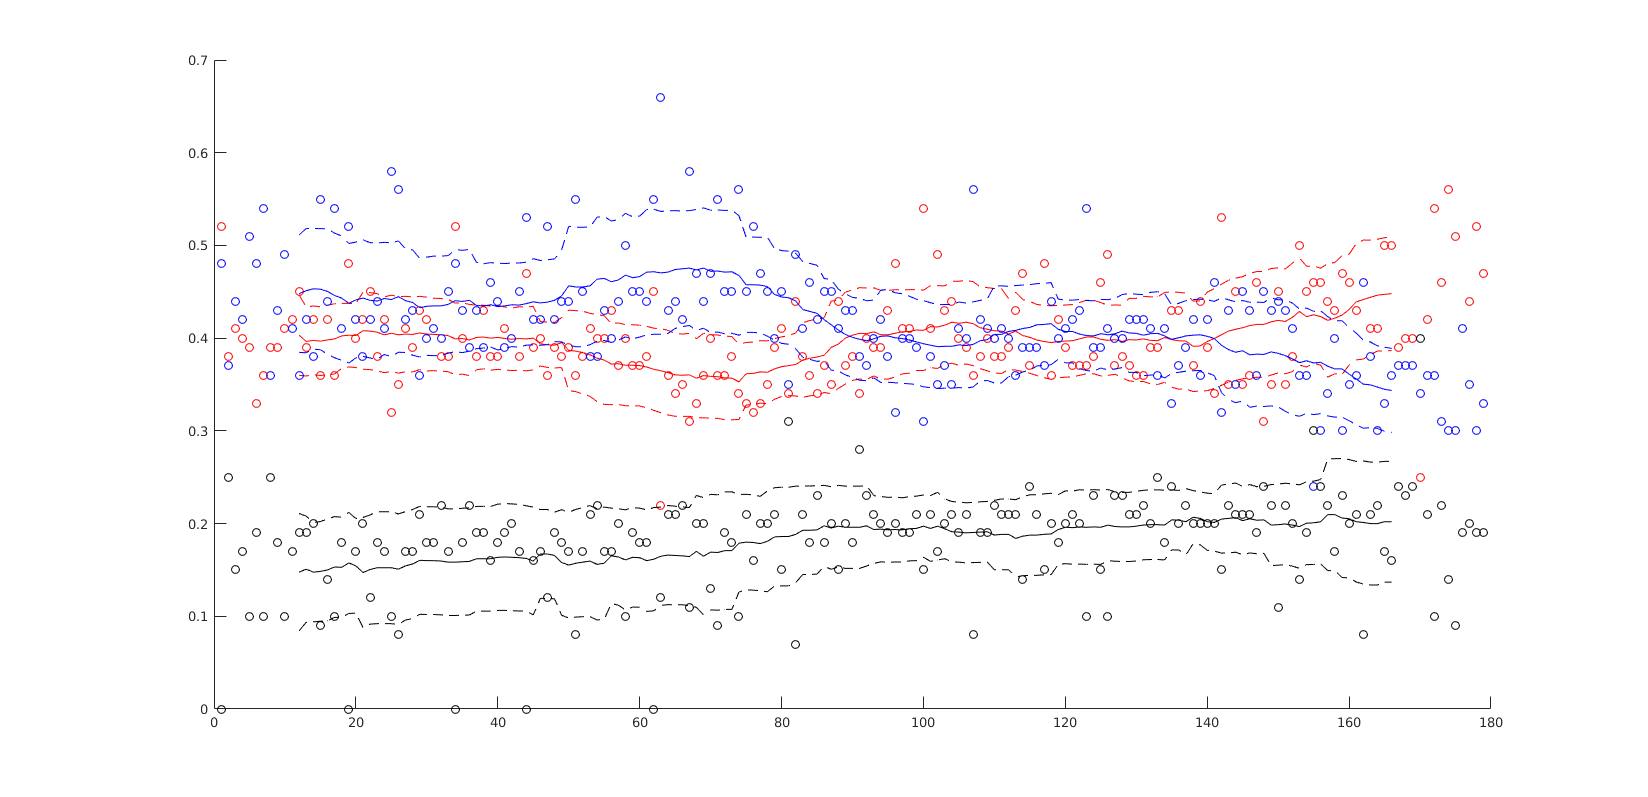
\includegraphics[width=0.8\textwidth]{./img/brexit.png}
\end{frame}

%%%%%%%%%%%%%%%%%%%%%%%%%%%%%%%%%%%%%%%%%%%%%%%%%%%%%%%%%%%%%%%%%%%%%%%%%%%%%%%
\begin{frame}[fragile]
  \frametitle{Example:  Brexit polling}

  \begin{Verbatim}
poll = csvread('brexit.csv');
% poll is a matrix. 
% In matlab, you can use 
% poll = importdata(’brexit.csv’);
% Then change below poll to be poll.data

n = numel(poll(:,3));
mean_l = rolling_mean( poll(:,3)', 25 );

fit_poly_l = polyfit( 13:167,mean_l(13:167),19 );  
poly_l = polyval( fit_poly_l,1:n );

hold on
plot( poll(:,3), 'ro' );
plot( 1:n,mean_l, 'r-' );
plot( 1:n,poly_l, 'r:' );
  \end{Verbatim}
\end{frame}

%%%%%%%%%%%%%%%%%%%%%%%%%%%%%%%%%%%%%%%%%%%%%%%%%%%%%%%%%%%%%%%%%%%%%%%%%%%%%%%
\begin{frame}[fragile]
  \frametitle{Polynomials}
  %\Enlarge

  \begin{enumerate}
  \myitem  Other equations are possible besides polynomials:
  \mysubitem  See the ``Nonlinear Least-Squares Curve Fitting in the Optimization Toolbox'' for more information.
  https://www.mathworks.com/help/optim/
  nonlinear-least-squares-curve-fitting.html
  \end{enumerate}
\end{frame}

%%%%%%%%%%%%%%%%%%%%%%%%%%%%%%%%%%%%%%%%%%%%%%%%%%%%%%%%%%%%%%%%%%%%%%%%%%%%%%%
\begin{frame}[fragile]
  \frametitle{Example:  Data fitting}

  \begin{Verbatim}
x = linspace( -2*pi,2*pi,21 );
y = sin( x );

figure; hold on;
plot( x,y,'.' );
for i = 2:9
    coefs = polyfit( x,y,i );
    xfit = linspace( -2*pi,2*pi,101 );
    yfit = polyval( coefs,xfit );
    plot( xfit,yfit,'-' );
end
  \end{Verbatim}
\end{frame}

% - PDE toolbox example?
% - find factorial using function browser

%%%%%%%%%%%%%%%%%%%%%%%%%%%%%%%%%%%%%%%%%%%%%%%%%%%%%%%%%%%%%%%%%%%%%%%%%%%%%%%%
\section{Reminders}

%%%%%%%%%%%%%%%%%%%%%%%%%%%%%%%%%%%%%%%%%%%%%%%%%%%%%%%%%%%%%%%%%%%%%%%%%%%%%%%%
\begin{frame}
  \frametitle{Reminders}
  \Enlarge

   \begin{itemize}
   	\myitem  Homework \#12 is due Friday, Jan.\ 13.  %\pause
   	%	\myitem  No lab \emph{t} week.  %\pause
   	\myitem  Final examination will be held Jan.\ 20, Friday 8am-11am in A-0414.  %\pause
   	% \myitem  Grade check period coming up:  Dec.\ 9--14.  \textcolor{CS101Base}{All Compass grades will be considered final after this.}
   \end{itemize}
\end{frame}

\end{document}
